\section{Evaluation}
In this section of the paper we will evaluate our work in real world applications and determine its strengths and weaknesses. We will use various implementation to perform this evaluation. We will also look into situations where the implementation does not match the protocol description and observe the systems behaviour.

%\subsection{Test Environment}
%For testing our 
\subsection{Chat Server}
To test the capabilities of our DSL, we decided to create a secure chat application. This application would allow  users to connect to the server and exchange secure and private messages with other connected users. We would establish a secure connection to the server and to each individual user that was connected using the DHM key exchange. This means that our Consumer needs to maintain a list of multiple private session keys and be able to determine which one to use for incoming messages.

One of the key benefits of this solution is that even though our central server will receive all the messages, they will be encrypted using two keys. The first key is the one that is established between the two consumers. The second key is the one that the Server and consumer created. This makes it impossible for the server to know what the actual content of the message is. All the server knows is who is talking to who. 

There will be two parts to a message, the headers and the actual text of the chat message. The headers will determine who the intended recipient is. Below we show an example chat message being sent from A to B.
$$
 \begin{multlined}
  \{\{Headers\}, \{Text\}Key_{A2B}\}Key_{A2Server}
 \end{multlined}
$$
Here we can see that the header is only encrypted with key between consumer A and the Server. The text however is encrypted by both the A2Server and A2B key. When the server receives this message, it decrypts it and forwards it to the correct recipient. It however re-encrypts the message using the B2Server key.
$$
 \begin{multlined}
  \{\{Headers\}, \{Text\}Key_{A2B}\}Key_{B2Server}
 \end{multlined}
$$
\\\\
The steps for the connecting client will be 3 steps. 
\begin{enumerate}
 \item Connect to the server and establish a secure communication channel
 \item Register our Username
 \item Receive and send chat messages
\end{enumerate}

Using the steps shown above we can create the protocol description for the server. 
\begin{lstlisting}[style=myScalastyle]
 val endpoint = new ProtocolBuilder()
 val dhm   = endpoint receives primeAndGenerator 
                  sends aPublicKey receives aPublicKey
 val chatServer = dhm receives aUsername 
                       next endpoint anyone aChatMessage loop()
\end{lstlisting}
Here we have re-used our implementation of DHM we defined earlier and added the messages needed for a chat server.

\subsubsection{Detection of Implementation Errors}
The main purpose of our DSL is to discover errors in implementation. When errors occur, we send the error generated by the Validator to the consumer. These errors will provide us with the information  we need to correct the implementation. 

It is up to the consumer to chose how to handle this error. In our implementation we simply print the error message to the terminal. When we run our application, we will be alerted whenever a error occurs and get the information we need to correct it.

We will show two of the errors we received when we where working on the implementation. One of the errors is when our validation failed. 
\begin{lstlisting}[style=myScalastyle]
  ``ValidationError(Msg could not be converted to a PrimeAndGenerator class: ,net.liftweb.json.MappingException: Do not know how to convert JString(239.0) into double)''
\end{lstlisting}
The first part of the message tells us where the error occurred. The second part is the actual exception that was generated. Using the first message we can see that the error ocurred in the message wrapping for PrimeAndGenerator. The exception tells us that we were unable to map ``JString(239)'' to a Double. This level of detail provides us with more than enough details to correct the error.

The second error we had was when our consumer had not implemented a case for the ``PrimeAndGenerator'' class in its the pattern matching.
\begin{lstlisting}[style=myScalastyle]
  ``Unspecified case for: PrimeAndGenerator(149.0,2.0)''
\end{lstlisting}

As we encounter these errors, we can quickly determine their cause and incrementally fix them until we have a running system. In this case we implemented a case for the PrimeAndGenerator where we continued the process defined in our protocol definition.

\subsubsection{Finished System}
After incrementally adding cases to our consumers pattern matching method, we ended up with a fully functioning system. In our implementation we made the clients chose a random integer as a username when connecting. 

The server alerts connected users when a new users connects. When the connected clients receive this ``NewUser'' alert, they establish a secure connection with the new user and send a simple greeting message. Below we have included the screen-shots of three terminals. The terminals represent the server (\ref{fig:server}), client A (\ref{fig:clienta}) and client B (\ref{fig:clientb}). In this scenario, client A is first to connect to the server and will send a greeting to client B.

\begin{figure}[H]
  \centering
  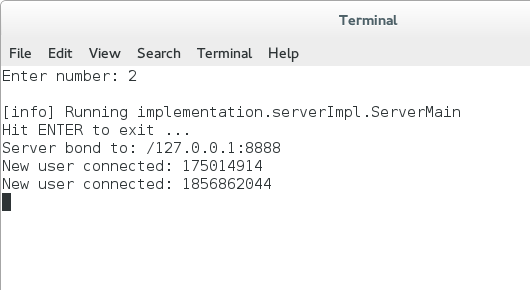
\includegraphics[width=1\linewidth]{evaluation/Server.png}
  \caption{Server}
  \label{fig:server}
\end{figure}

\begin{figure}[H]
  \centering
  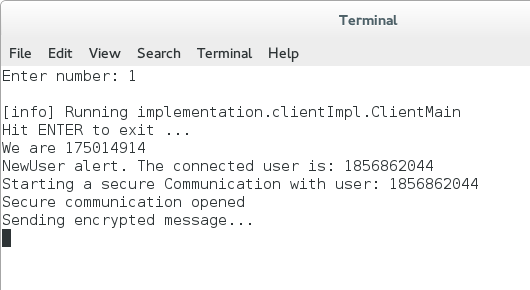
\includegraphics[width=1\linewidth]{evaluation/ClientA.png}
  \caption{Client A - Sends message}
  \label{fig:clienta}
\end{figure}

\begin{figure}[H]
  \centering
  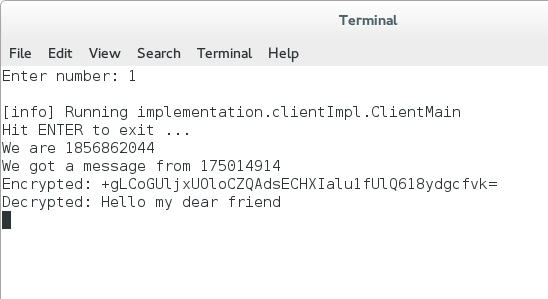
\includegraphics[width=1\linewidth]{evaluation/ClientB.png}
  \caption{Client B - Receives message}
  \label{fig:clientb}
\end{figure}

Any additional clients that connect to the server will also receive greeting messages from both client A and B.

%ServerSide => Unspecified case for: PrimeAndGenerator(149.0,2.0)

%ClientSide => ValidationError(Msg could not be converted to a PrimeAndGenerator class: ,net.liftweb.json.MappingException: Do not know how to convert JString(239.0) into double)


%Server Username => Unspecified case for: LPO2gbvztUktNyx5+BIsidWgBKslDau969BoddEUcs8=

\subsection{Measuring Performance}
To measure the performance of our system, we have decided to implement echo servers that both use and don't use our system.

By using our DSL we will check if every single message sent or received obeys a given protocol. This involves checking that the message contents and protocol specification are of an expected value. These extra steps do not come for free and the overall throughput of the system should be lower than that of a system with no such checking. 

To test this we have created 3 implementations that all build upon the previous implementation. The implementations will be on the server side and will all provide an echo server. The three implementations are the following:

\begin{description}
  \item[Basic] does not use a PM and sends data directly to the consumer
  \item[Uses PM] uses our PM with a simple String Validator
  \item[Wrapping] the Validator wraps messages into an EchoMessage class
\end{description}
We have created a client that measures the time it takes to send and receive a given amount of messages.

The data below shows the average scores for the implementations. As there is some overhead costs when connecting to the server and sending the first message, we do not disconnect and reconnect for each iteration. Instead, we count the time it took to receive the first 10000, 20000, 30000 etc. messages. We gathered results from 20 such iterations. The results below in table \ref{tab:performance} are the averages for each iteration. The time is given in milliseconds. 

\begin{table}[h]
	\centering
	\begin{tabular}{|l|l|l|}
		\hline
		{\bf }         & {\bf Average} & {\bf Message/ms} \\ \hline
		{\bf Basic}    & 489           & 20.40              \\ \hline
		{\bf Uses PM}  & 544           & 18.37              \\ \hline
		{\bf Wrapping} & 589           & 16.37              \\ \hline
	\end{tabular}
	\label{tab:performance}
	\caption{Average performance of implementations given in milliseconds}
\end{table}
% Uses PM is perhaps the most comparable one
If we look at the data we can see quite clearly that there is a performance penalty when using our system. Analysing the performance table we can see that the throughput of the system is reduced by approximately 4 messages in the full implementation that uses wrapping. Sending 10000 round-trip message that bypasses the PM took an average of 489 milliseconds. Messages that went through the PM and were wrapped took on average 589 milliseconds. This is an increase of approximately 20\%. In many application this increase could potentially be unacceptable. 


\subsubsection{Analysing the performance drop}
The reason why the Basic implementation is faster is that it does not need to read the data it receives. It simply returns whatever it receives, without looking at the contents. The other implementations need to perform several additional steps than just echoing the message:
\begin{enumerate}
  \item Check if receiving is according to the protocol state
  \item Update protocol state
  \item Convert the message to a String 
  \item Validate the message
  \item Send validated message to the Consumer
  \item Generate and send response
  \item Check if sending is according to the protocol state
  \item Validate the message
  \item Update protocol state
  \item Convert message to a ByteString
  \item Send the message
\end{enumerate}
As we can see there are quite a few additional steps involved in our system. It seems only natural that the we would suffer from some form of performance loss.

We feel however that a 20\% cost is acceptable for most applications as we are comparing it to a system that has no checking and does not abide by any type of protocol. In addition, this DSL is not focused on performance, but increasing readability, maintainability and helping with the implementation. If we had more time we could tweak our system to offer better performance, but this was never a high priority during design. 


\subsection{Bug Discovery}

While running performance test we stumbled upon what we believed to be a bug inside the DSL itself. After the performance testing client had sent around 70 000 messages to the server, it would have a protocol failure. The error was that the server was receiving a message, while the protocols state was in a sending state. We found this strange as the client only sends a message after it has received a message. As our test client was such a simple implementation, we believed the error was perhaps located somewhere within the DSL.
 
After some debugging of the system, we discovered that the bug was in fact withing the testing client. In our implementation we were accidentally sending an extra message to the server when restarting our counter. After several restarts, the accumulated additional messages would eventually arrive before the server had sent a response.

This error was not discovered when we tested the ``Basic'' implementation, so we had to rerun our performance test for it. This error was only discovered as we were stress testing the system and would most likely not have of been caught if were sending a lower amount of messages.


\subsection{Building DSLs with Scala}
Scala is a powerful language that provides us with much freedom in our creation of a DSL. This freedom is however restrictive in certain areas. Many of these restrictions have been discussed in Section \ref{sec:scala} Scala.
 
The perhaps most interesting question when evaluating Scala as a host language for a DSL is to ask if it ever got in the way of implementing our DSL the way we wanted to. To answer this question we consider what we would change in our DSL if Scala did not have any restrictions. At the moment of writing, we do not believe that any of the restrictions that Scala has have affected our implementation negatively. If anything our DSL has not taken advantage of the features offered by Scala. Specifically we could use more implicit values and features such as currying \cite{odersky2008programming}. 


\subsection{Weaknesses}
We have identified what we believe to be some of the main weaknesses with this DSL.

The first is the performance loss of approximately 20\%. The performance test was however slightly unfair as the we compared our system to a system with absolutely no wrapping or any data manipulation. We can therefor consider the 20\% loss as the worst case scenario for similar solutions.

The second weakness is specifying protocols that involve more than 2 participants. By using the Event Bus provided by Akka, we are able to enable communication among the consumers, but this communication channel is not necessarily regulated by a Validator. Sending internal messages that are not defined in the protocol specification can cause undesired side-effects. 

A third weakness is that the system provides no constructs for dealing with packet loss in the network. In real work applications packets may travel different paths in the network to reach their target. This means that they can be sent in the correct order, but arrive in an alternative order.

Our final weakness is that there is no indication of error when a consumer should send a message, but is idle. For example, if our echo server does not respond to a echo message, no error would occur. It would only be noticed by the client that would never receive a response. 

%Even though you implement the DSL, there is no guarantee that it will help debugging the implementation. This is because the strengths of this DSL are heavily dependant on the developers and how they decide to implement a network protocol. Although the use of validators provide a clean way of separating concerns in a system, they must be implemented correctly. Poorly written error messages will not provide useful information when debugging. Validators must try to encapsulate as much of the systems complexity as possible. This complexity should be the focus of determining the purpose of a message and wrapping it in a suitable case class. In most cases, the validator should wrap messages inside classes. This will greatly help building the consumers pattern matching function.


\subsection{Accomplished Objectives}
All the objectives have been met, with the exception of the tertiary ones. One of the secondary objective was to be able to implement additional protocols, specifically the Needham-Schroeder protocol. The main difference of this protocol compared to the Diffie-Hellman-Merkel protocol is that it involves direct communication with multiple clients. With our DHM key exchange, HTTP server and chat server implementations, we only have direct communication with a single client.

To solve multiple connections we must use the Event Bus to communicate with the other actors. In Needham-Schroeder we need direct communication with a server and a client. Figure \ref{fig:Needham} shows an example of how we could implement the protocol. 

\begin{figure}[H]
  \centering
  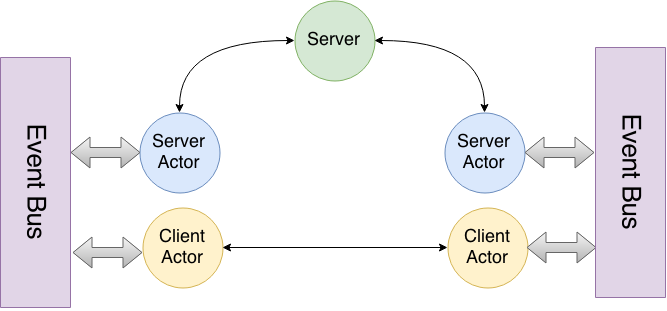
\includegraphics[width=1\linewidth]{evaluation/Needham.png}
  \caption{Needham-Schroeder Actors}
  \label{fig:Needham}
\end{figure}

Here we can create a PM for both the Server and Client actors. This way the PM will be responsible only for communication over a single channel with two participants. The Server and Client actors communicate over the event bus, allowing them to exchange the messages they receive from their connections.

Using similar solutions, we should be able to implement a multitude of different protocols.

 
\iffalse
If you meet your objectives
How did I test it
How do I know its working What happens when it goes wrong
--- Draft 3 ---
How well were the objectives met
What is the performance compared to no checking
-Does not need to quantifiable
How secure it is
How we set out writing it?
"  made this thing using my DSL"
Performance with different message sizes

Speculate on why a sys is slow



Is scala a good language for building a DSL?

This approach definatly has merrits...


Errors: 

ServerSide => Unspecified case for: PrimeAndGenerator(149.0,2.0)

ClientSide => ValidationError(Msg could not be converted to a PrimeAndGenerator class: ,net.liftweb.json.MappingException: Do not know how to convert JString(239.0) into double)


Server Username => Unspecified case for: LPO2gbvztUktNyx5+BIsidWgBKslDau969BoddEUcs8=
\fi

